This section details the experimental methodology, including the dataset employed, the procedures for data pre-processing and synthetic fault injection, and the architecture of our proposed Hierarchical Fault Identification Network (HiFiNet) for fault classification in WSNs.

\subsection{Dataset}
\subsubsection{Data Source}
The dataset used in this study is the Intel Lab Dataset. This dataset comprises readings from a network of 54 sensor nodes, specifically Mica2Dot devices, which were outfitted with environmental sensing capabilities. These nodes systematically captured time-stamped information relating to ambient conditions, including temperature, humidity, light levels, and the sensors' own voltage. The data acquisition process occurred at intervals of roughly 31 seconds for each sensor. The collection period for this particular dataset extended from late February 2004 through early April 2004 \cite{Intel2004}.

\subsubsection{Fault Injection}
To evaluate the performance of HiFiNet in classifying various fault types, synthetic faults were injected into the pre-processed normal temperature data. 

For each experimental dataset created, faults were injected such that within the selected subset of six nodes (nodes 7-12), five nodes were each assigned a distinct fault type, and one node remained normal (i.e., its data was not corrupted). This setup allows for the analysis of one specific fault type per sensor in the context of other faulty and normal sensors.

Multiple datasets were generated with varying overall percentages of faulty instances, specifically 5\%, 10\%, 15\%, and 20\% of the total data points being faulty. Within each dataset, the total fault rate was divided equally among the five predefined fault types. Faults were injected based on their mathematical models (as described in Section \ref{subsec:types}). In total, 4 datasets are created corresponding to each fault rate.

The time series sequences were labeled with a specific fault type if any sample within that sequence contained the corresponding injected fault. This creates a labeled dataset suitable for supervised learning.

\subsection{Hierarchical Fault Identification Network (HiFiNet)}
\begin{figure}[htbp]
  \centering
  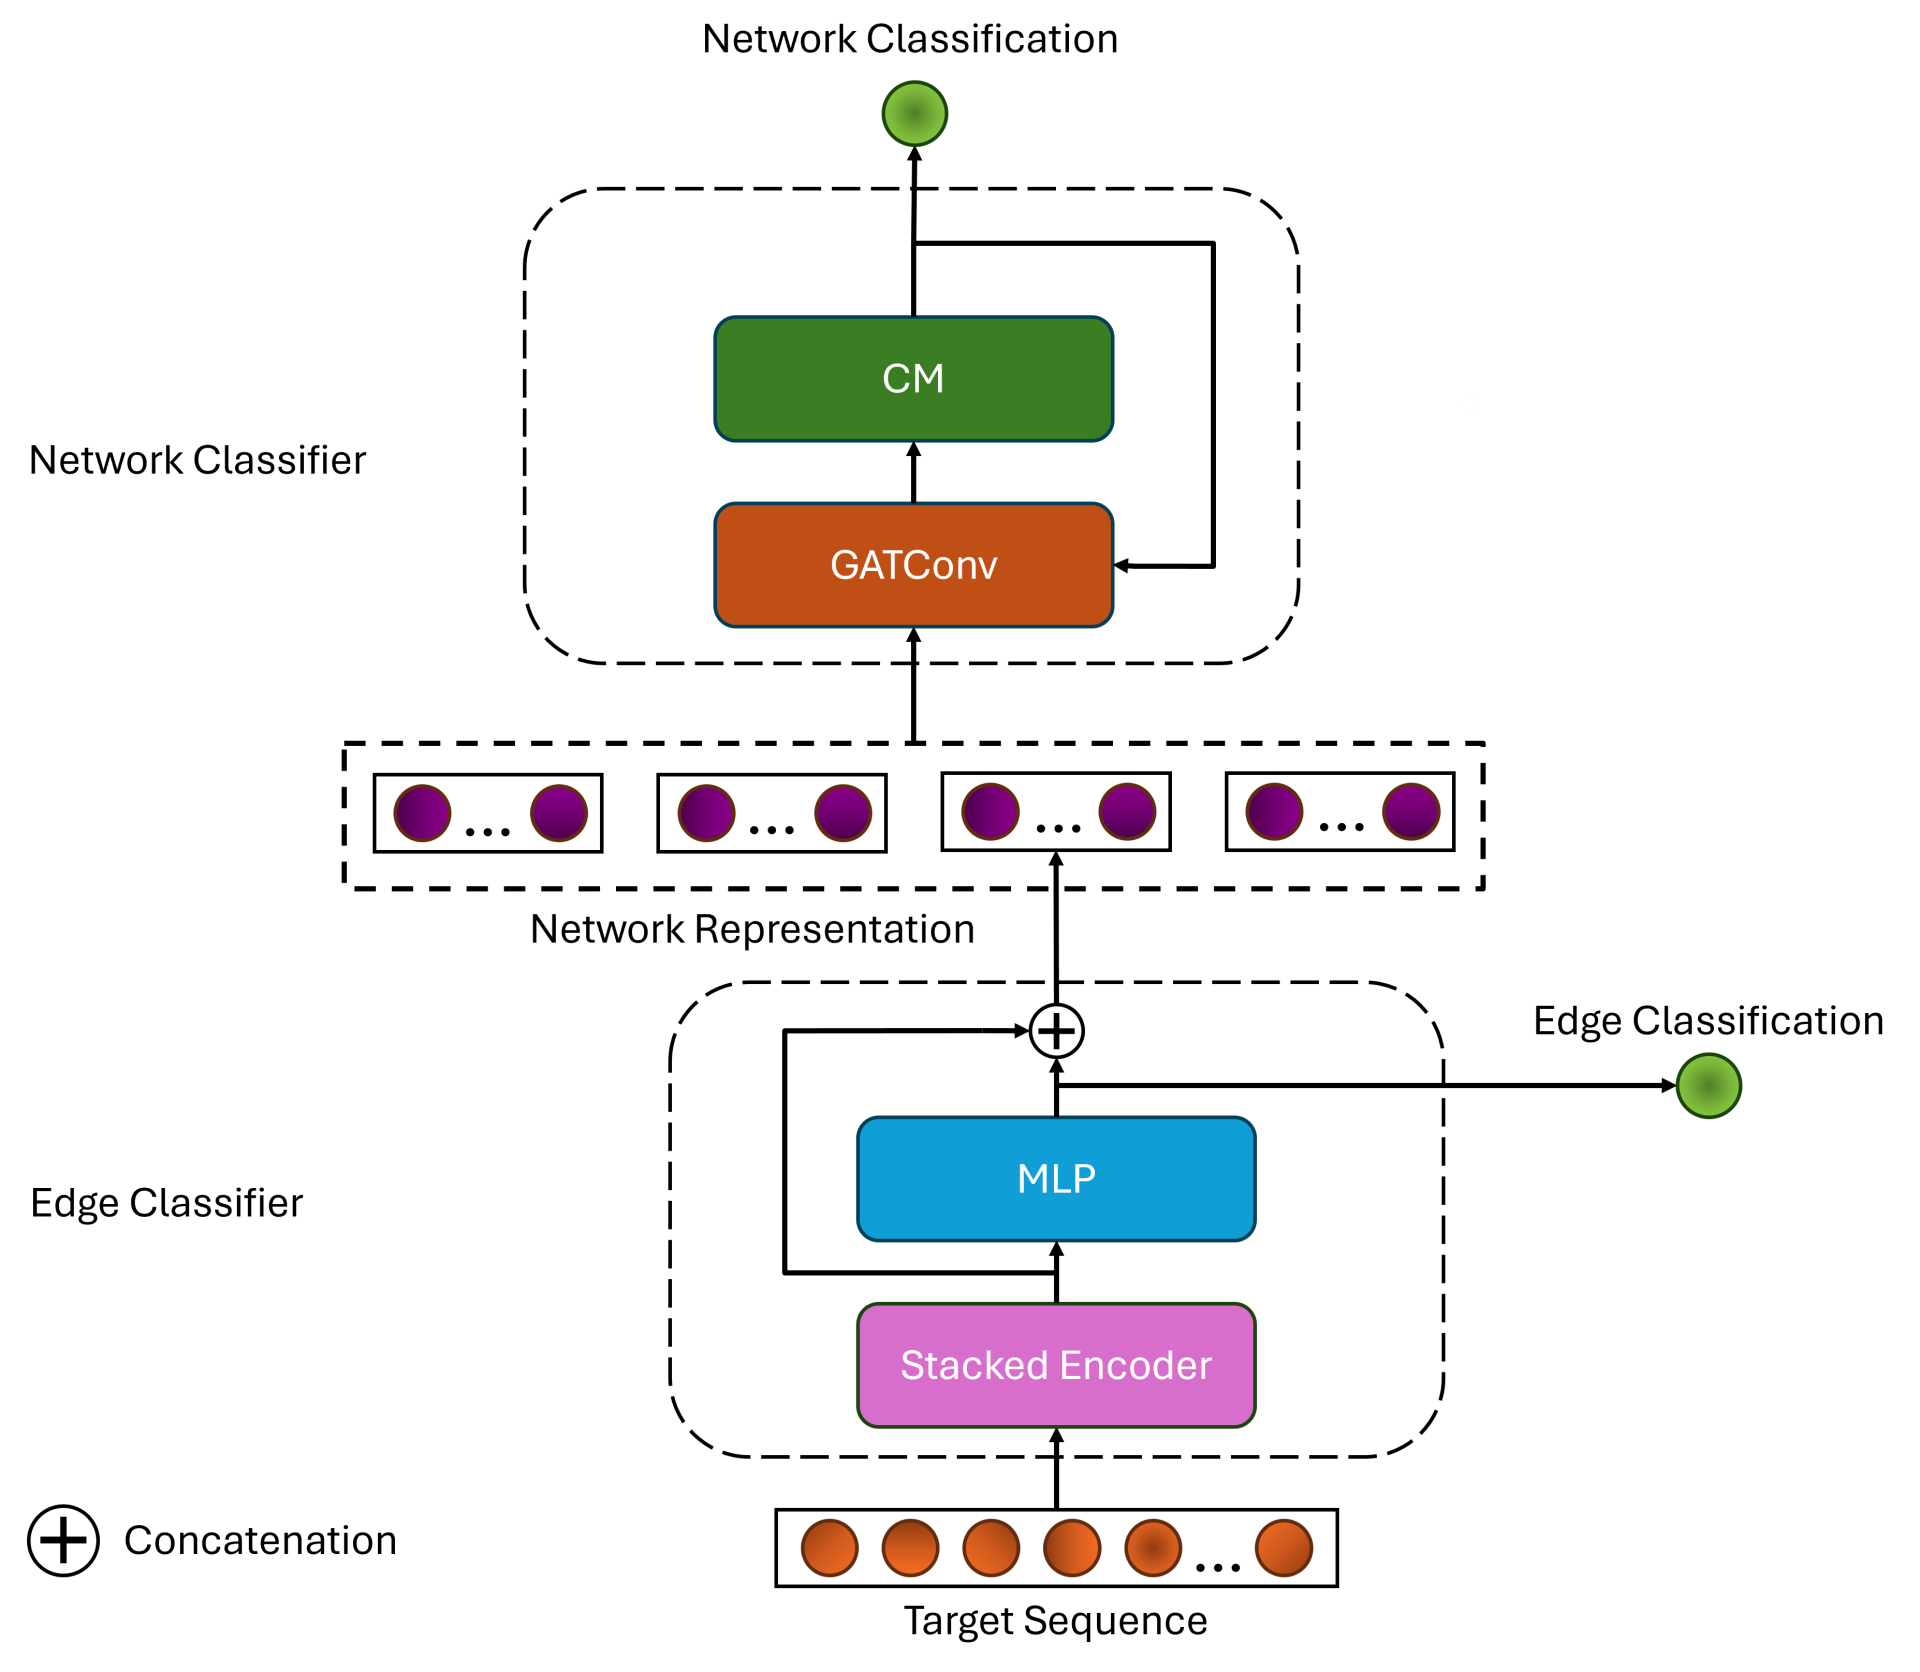
\includegraphics[width=0.8\linewidth]{images/HiFiNet.png}
  \caption{Proposed HiFiNet model, illustrating the Edge Classifier processing a target node's temperature sequence and the Network Classifier integrating edge outputs with contextual network data.}
  \label{fig:hifinet}
\end{figure}
We propose HiFiNet, a Hierarchical Fault Identification Network, for the classification of sensor faults in WSNs. The architecture, depicted in Figure \ref{fig:hifinet}, employs a two-stage hierarchical approach to classify faults, leveraging both individual sensor data and contextual information from the network.

\subsubsection{Edge Classifier}
The first stage of HiFiNet is the Edge Classifier, which focuses on analyzing the time series data from an individual target sensor node to extract discriminative features and perform an initial fault classification. The design of the Edge Classifier involves a two-phase training process: unsupervised pre-training of a feature extractor using a LSTM-SAE architecture, followed by supervised fine-tuning for the fault classification task.
\begin{itemize}
  \item Phase 1: Unsupervised Pre-training with LSTM-SAE 

  The feature-extraction component is built from an LSTM-SAE with encoder layers. This autoencoder is trained in an unsupervised, layer-wise fashion to learn compressed representations of~\(X_w\).

  \begin{itemize}
    \item \emph{Layer \(l=1\):}
      \[
        \begin{aligned}
          H_1 &= E_1\bigl(X_w;\,\theta_{E_1}\bigr), \\
          \hat X_w &= D_1\bigl(H_1;\,\theta_{D_1}\bigr) \\
        \end{aligned}
      \]

      With \(E_1\) and \(D_1\) being the first encoder and decoder layer, and \(\theta_{E_1}\), \(\theta_{D_1}\) being their parameters respectively.
      \[(\hat\theta_{E_1},\,\hat\theta_{D_1}) = \underset{\theta_{E_1}, \theta_{D_1}} {\arg\min} \mathcal L_{\mathrm{recon}}\bigl(X_w,\;\hat X_w\bigr).\]
  \end{itemize}
\end{itemize}
